\begin{figure}
    \centering
    

\tikzset{every picture/.style={line width=0.75pt}} %set default line width to 0.75pt        

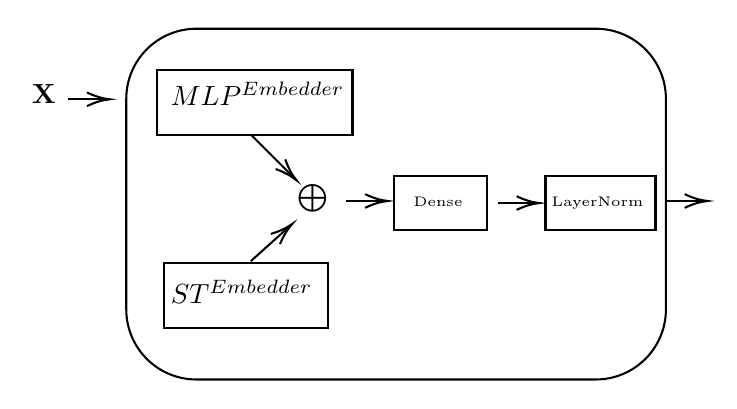
\begin{tikzpicture}[x=0.75pt,y=0.75pt,yscale=-1,xscale=1]
%uncomment if require: \path (0,300); %set diagram left start at 0, and has height of 300

%Straight Lines [id:da9383935885348577] 
\draw    (110,97) -- (128,97) ;
\draw [shift={(130,97)}, rotate = 180] [color={rgb, 255:red, 0; green, 0; blue, 0 }  ][line width=0.75]    (10.93,-3.29) .. controls (6.95,-1.4) and (3.31,-0.3) .. (0,0) .. controls (3.31,0.3) and (6.95,1.4) .. (10.93,3.29)   ;
%Shape: Rectangle [id:dp26157196515791103] 
\draw   (267,134) -- (312,134) -- (312,160) -- (267,160) -- cycle ;
%Straight Lines [id:da3903825796548569] 
\draw    (244,146) -- (262,146) ;
\draw [shift={(264,146)}, rotate = 180] [color={rgb, 255:red, 0; green, 0; blue, 0 }  ][line width=0.75]    (10.93,-3.29) .. controls (6.95,-1.4) and (3.31,-0.3) .. (0,0) .. controls (3.31,0.3) and (6.95,1.4) .. (10.93,3.29)   ;
%Straight Lines [id:da31519440110945307] 
\draw    (317,147) -- (335,147) ;
\draw [shift={(337,147)}, rotate = 180] [color={rgb, 255:red, 0; green, 0; blue, 0 }  ][line width=0.75]    (10.93,-3.29) .. controls (6.95,-1.4) and (3.31,-0.3) .. (0,0) .. controls (3.31,0.3) and (6.95,1.4) .. (10.93,3.29)   ;
%Rounded Rect [id:dp5570244485049601] 
\draw   (138,96.8) .. controls (138,78.13) and (153.13,63) .. (171.8,63) -- (364.2,63) .. controls (382.87,63) and (398,78.13) .. (398,96.8) -- (398,198.2) .. controls (398,216.87) and (382.87,232) .. (364.2,232) -- (171.8,232) .. controls (153.13,232) and (138,216.87) .. (138,198.2) -- cycle ;
%Straight Lines [id:da4015834386088226] 
\draw    (198,114) -- (218.59,134.59) ;
\draw [shift={(220,136)}, rotate = 225] [color={rgb, 255:red, 0; green, 0; blue, 0 }  ][line width=0.75]    (10.93,-3.29) .. controls (6.95,-1.4) and (3.31,-0.3) .. (0,0) .. controls (3.31,0.3) and (6.95,1.4) .. (10.93,3.29)   ;
%Shape: Rectangle [id:dp24629861152440957] 
\draw   (153,83) -- (247,83) -- (247,114) -- (153,114) -- cycle ;
%Shape: Rectangle [id:dp5370044089756952] 
\draw   (156,176) -- (235,176) -- (235,207) -- (156,207) -- cycle ;
%Straight Lines [id:da2688768933858873] 
\draw    (198,175) -- (216.51,158.34) ;
\draw [shift={(218,157)}, rotate = 138.01] [color={rgb, 255:red, 0; green, 0; blue, 0 }  ][line width=0.75]    (10.93,-3.29) .. controls (6.95,-1.4) and (3.31,-0.3) .. (0,0) .. controls (3.31,0.3) and (6.95,1.4) .. (10.93,3.29)   ;
%Shape: Rectangle [id:dp657610333809877] 
\draw   (340,134) -- (393,134) -- (393,160) -- (340,160) -- cycle ;
%Straight Lines [id:da9924932365682823] 
\draw    (398,146) -- (416,146) ;
\draw [shift={(418,146)}, rotate = 180] [color={rgb, 255:red, 0; green, 0; blue, 0 }  ][line width=0.75]    (10.93,-3.29) .. controls (6.95,-1.4) and (3.31,-0.3) .. (0,0) .. controls (3.31,0.3) and (6.95,1.4) .. (10.93,3.29)   ;

% Text Node
\draw (158,182.4) node [anchor=north west][inner sep=0.75pt]    {$ST^{Embedder}$};
% Text Node
\draw (158,87.4) node [anchor=north west][inner sep=0.75pt]    {$MLP^{Embedder}$};
% Text Node
\draw (219,136.4) node [anchor=north west][inner sep=0.75pt]    {$\bigoplus $};
% Text Node
\draw (91,88.4) node [anchor=north west][inner sep=0.75pt]    {$\mathbf{X}$};
% Text Node
\draw (275,142.5) node [anchor=north west][inner sep=0.75pt]   [align=left] {{\tiny Dense}};
% Text Node
\draw (341.5,142.5) node [anchor=north west][inner sep=0.75pt]   [align=left] {{\tiny LayerNorm}};


\end{tikzpicture}
    \caption{Encoder overview}
    \label{fig:gnn-encoder}
\end{figure}